\documentclass[svgnames,11pt]{beamer}
\input{/home/tof/Documents/Cozy/latex-include/preambule_commun.tex}
\input{/home/tof/Documents/Cozy/latex-include/preambule_beamer.tex}
%\usepackage{pgfpages} \setbeameroption{show notes on second screen=left}
\author[]{Christophe Viroulaud}
\title{Réseau internet}
\date{\framebox{\textbf{Int 01}}}
%\logo{}
\institute{Seconde - SNT}

\begin{document}
\begin{frame}
\titlepage
\end{frame}
\begin{frame}
    \frametitle{}
    D'après le site \emph{Internet Live Stats}, plus de 4,79 milliards de personnes dans le monde avaient accès à Internet fin 2020.
    
\begin{framed}
    \centering Comment connecter plusieurs machines ensemble?
\end{framed}
\end{frame}
\section{Historique}
\begin{frame}
    \frametitle{Historique}

    \begin{center}
    \centering
    
\includegraphics[width=6cm]{ressources/darpa.png}
    \captionof{figure}{\centering \textbf{Octobre 1962:} La DARPA (Defense Advanced Research Projects Agency) recrute Joseph Licklider comme le premier chef du programme de recherche en informatique.}
    \label{IMG}
    \end{center}
\note{Licklider: concept réseau galactique: relier ordinateurs}
\end{frame}
\begin{frame}

    \begin{center}
    \centering
    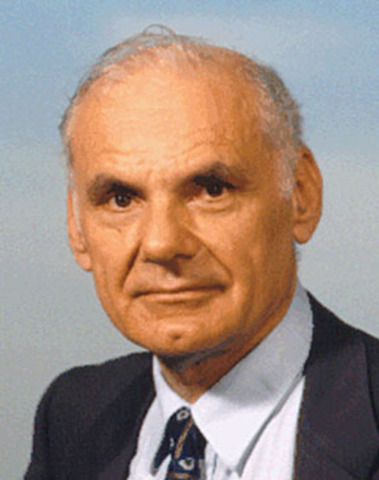
\includegraphics[width=4cm]{ressources/roberts.jpg}
    \captionof{figure}{\centering \textbf{1967:} Lawrence Roberts fut engagé par la DARPA pour développer le concept de réseau informatique. Il mit rapidement en place son plan pour le réseau \textbf{ARPANET}}
    \label{IMG}
    \end{center}

\end{frame}
\begin{frame}

    \begin{center}
    \centering
    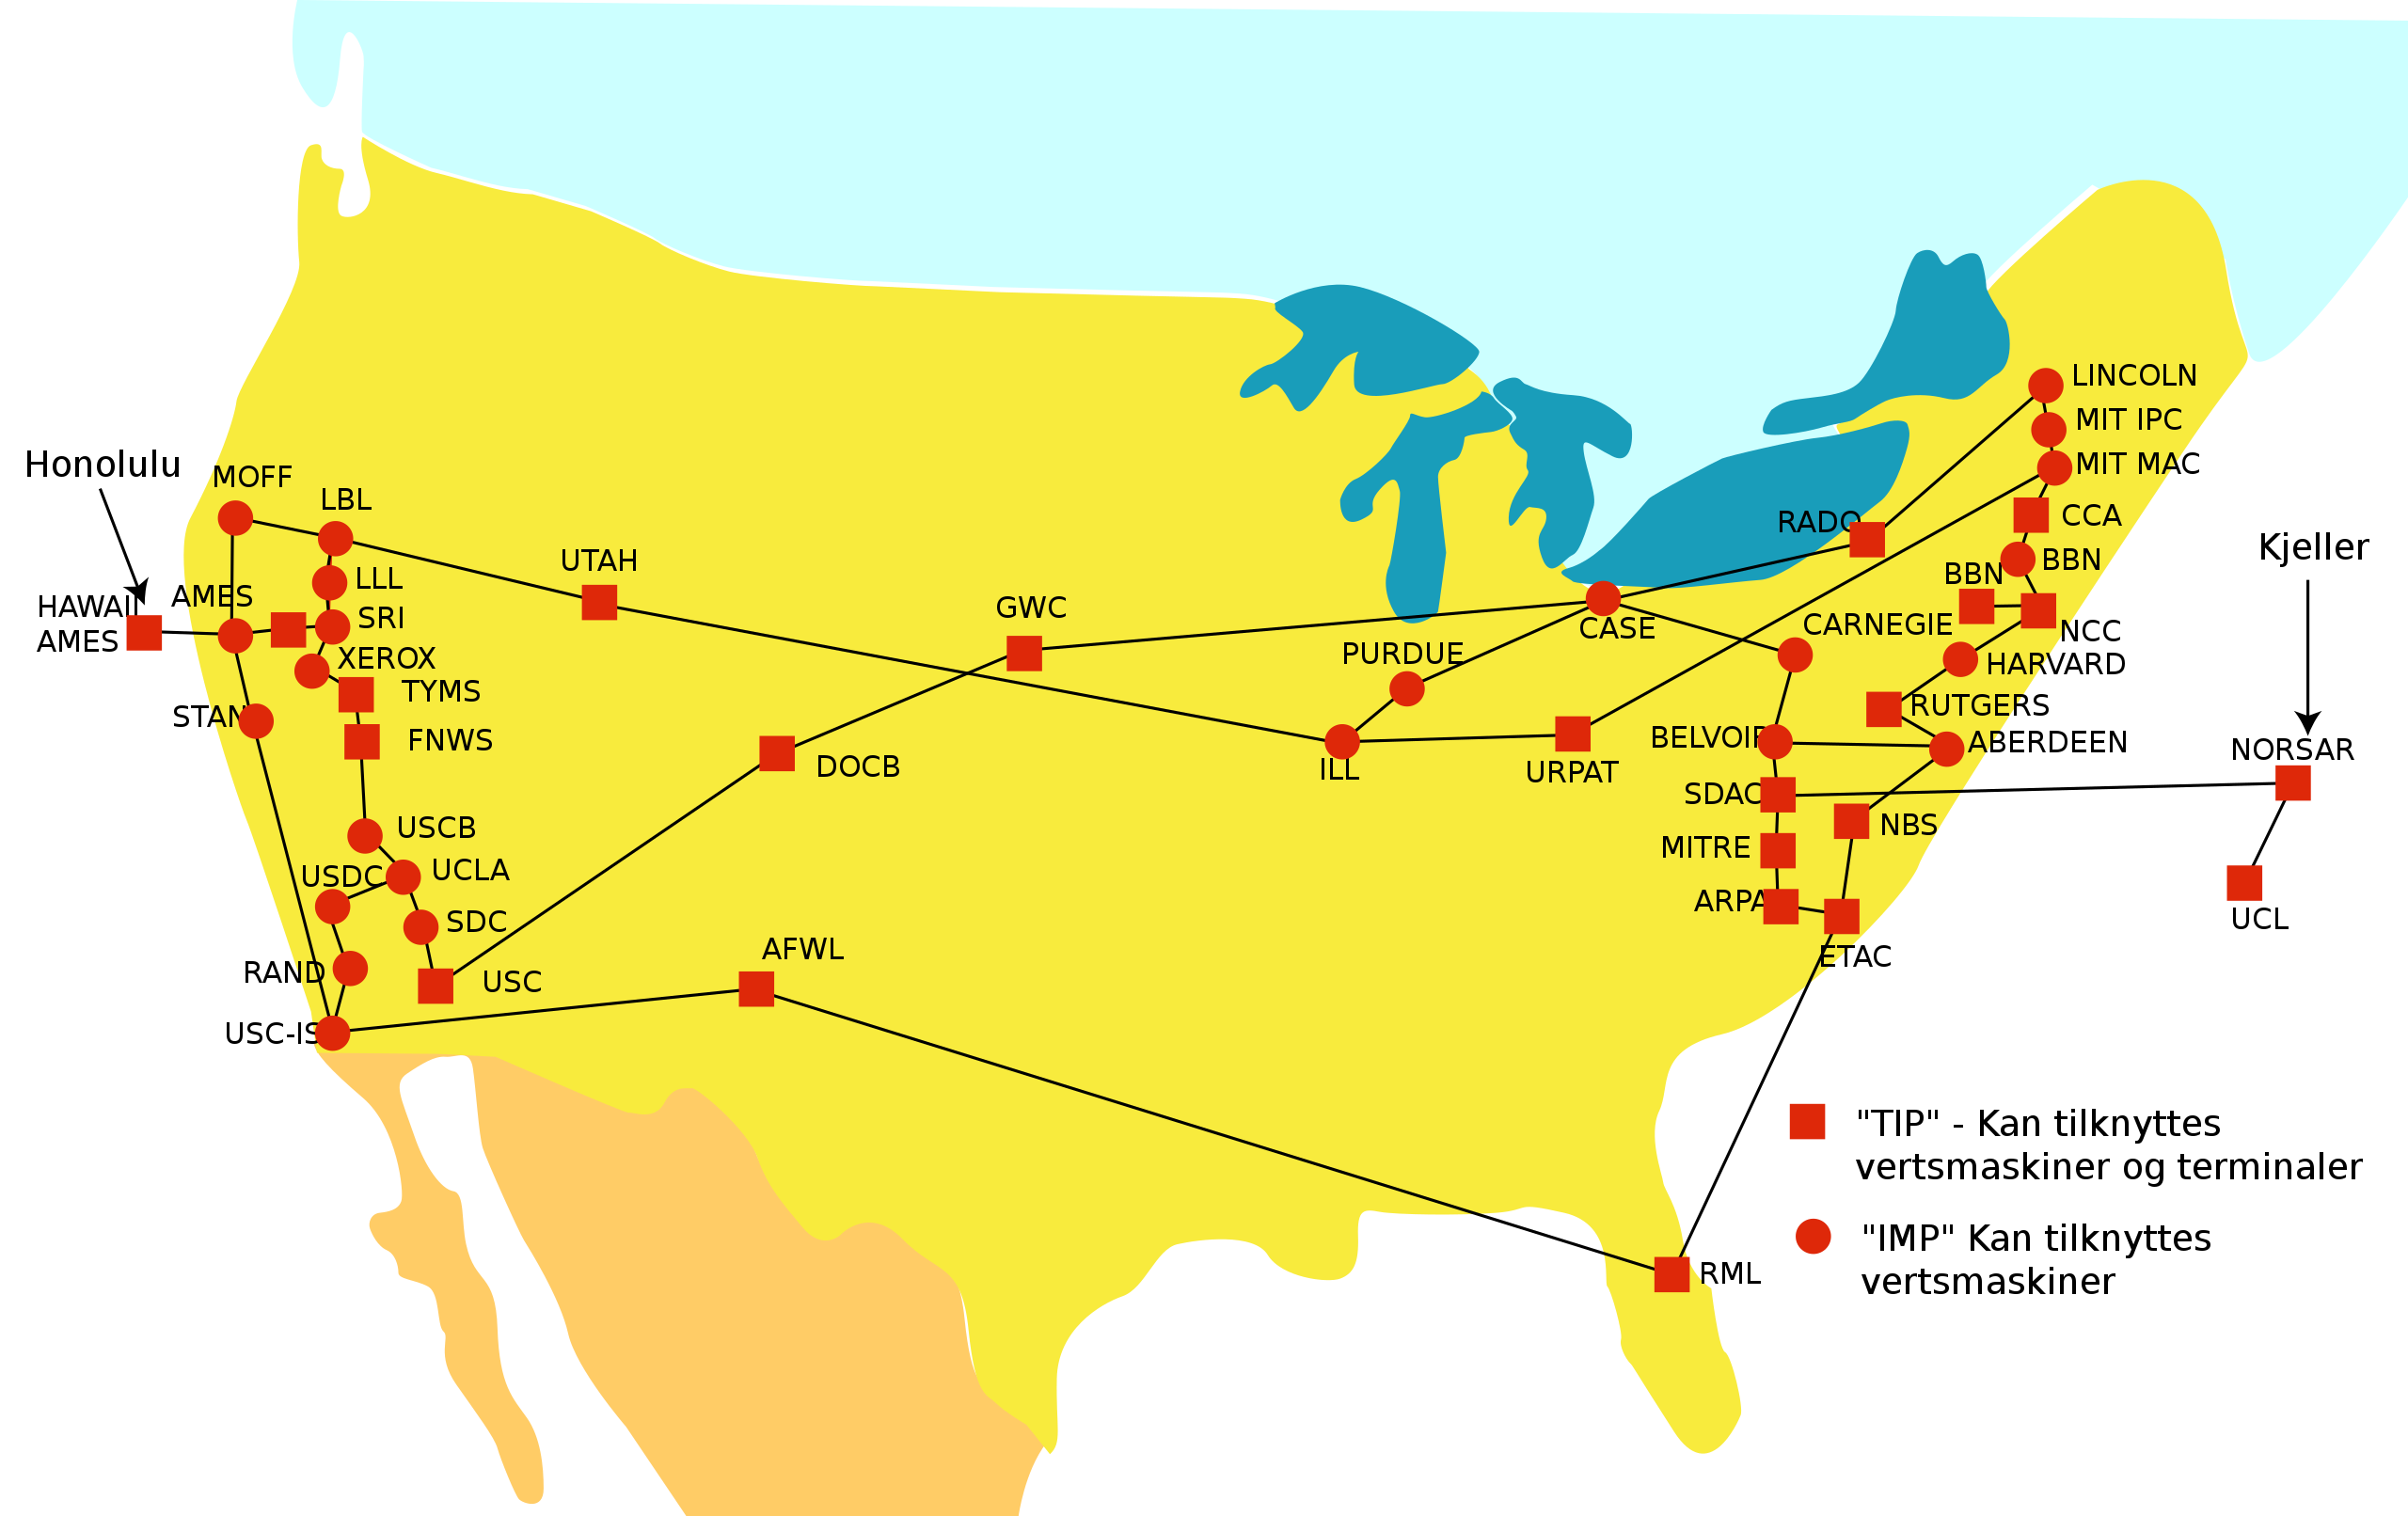
\includegraphics[width=8cm]{ressources/arpanet.png}
    \captionof{figure}{\centering \textbf{Octobre 1972:} Première démonstration publique du réseau ARPANET}
    \label{IMG}
    \end{center}

\end{frame}
\begin{frame}
    \frametitle{}

    \begin{aretenir}[]
    Le réseau ARPANET est composé de:
    \begin{itemize}
        \item 4 nœuds en 1969 (ouest des États-Unis),
        \item 23 nœuds en 1971, 
        \item 111 nœuds en 1974.
    \end{itemize}
    Il relie principalement des universités américaines.
    \end{aretenir}

\end{frame}
\begin{frame}

    \begin{center}
    \centering
    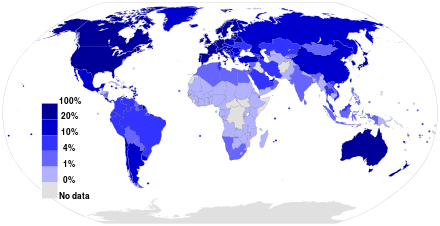
\includegraphics[width=8cm]{ressources/internet.png}
    \captionof{figure}{\centering \textbf{1983:} Le réseau ARPANET est séparé en un réseau militaire et un réseau publique: le terme \textbf{Internet} est adopté.}
    \label{IMG}
    \end{center}

\end{frame}
\begin{frame}

    \begin{center}
    \centering
    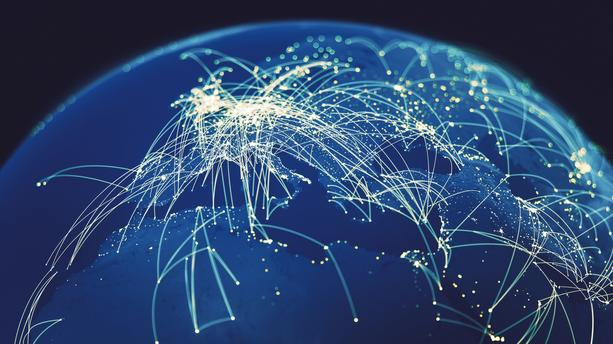
\includegraphics[width=8cm]{ressources/connexion.jpeg}
    \captionof{figure}{\centering Nombre d'ordinateurs connectés:
    }
    \label{IMG}
    \end{center}
    \begin{itemize}
        \item \textbf{1984: }mille ordinateurs,
        \item \textbf{1987: }dix mille ordinateurs,
        \item \textbf{1989: }cent mille ordinateurs,
        \item \textbf{1992: }un million d'ordinateurs.
    \end{itemize}
\end{frame}
\section{Réseau local}
\begin{frame}
    \frametitle{Réseau local}
\begin{center}
\centering
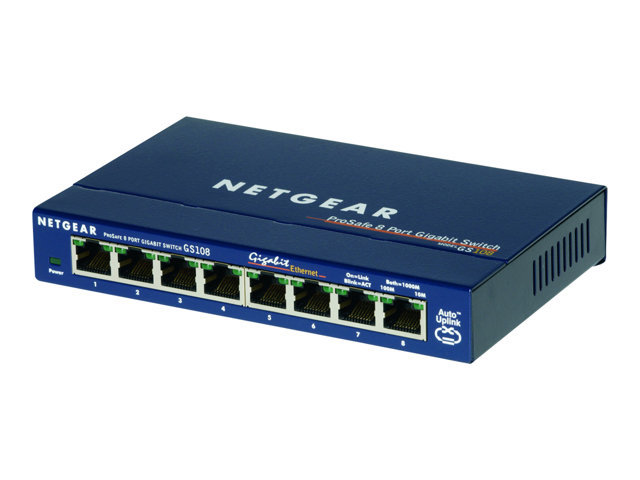
\includegraphics[width=8cm]{ressources/switch.jpg}
\captionof{figure}{\centering Pour relier plusieurs ordinateurs entre eux on peut utiliser un \textbf{commutateur (switch)}.}
\label{IMG}
\end{center}

\end{frame}
\begin{frame}
    \frametitle{}

\begin{center}
\centering
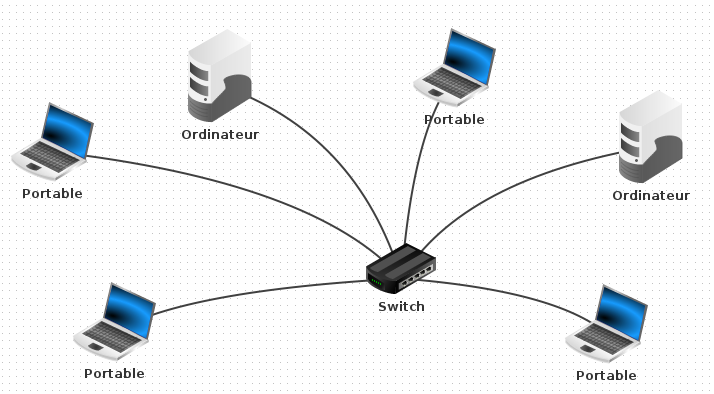
\includegraphics[width=8cm]{ressources/local.png}
\captionof{figure}{\centering \textbf{Réseau en étoile: }Le commutateur dirige les informations d'une machine à l'autre.}
\label{IMG}
\end{center}

\end{frame}
\begin{frame}
    \frametitle{}

    \begin{activite}
    \begin{enumerate}
        \item Simuler la structure en étoile.
        \item Déterminer les avantages et les inconvénients de ce type de réseau.
    \end{enumerate}
    \end{activite}

\end{frame}
\begin{frame}
    \frametitle{}

    \begin{aretenir}[]
    Un réseau en étoile est simple et peu coûteux à mettre en place. Cependant, il ne peut être utilisé que pour un \textbf{réseau local} de petite taille.
    \end{aretenir}

\end{frame}
\section{Réseau Internet}
\subsection{Structure maillée}
\begin{frame}
    \frametitle{Réseau Internet - Structure maillée}

    \begin{center}
    \centering
    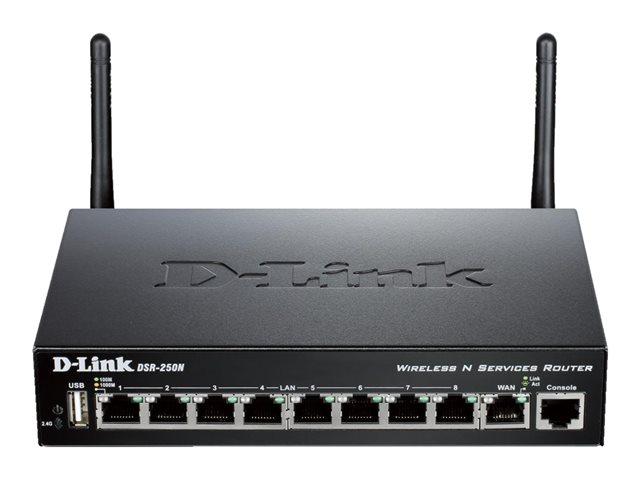
\includegraphics[width=8cm]{ressources/routeur.png}
    \captionof{figure}{Un \textbf{routeur} relie plusieurs réseaux entre eux.}
    \label{IMG}
    \end{center}

\end{frame}
\begin{frame}
    \frametitle{}

    \begin{center}
        \centering
        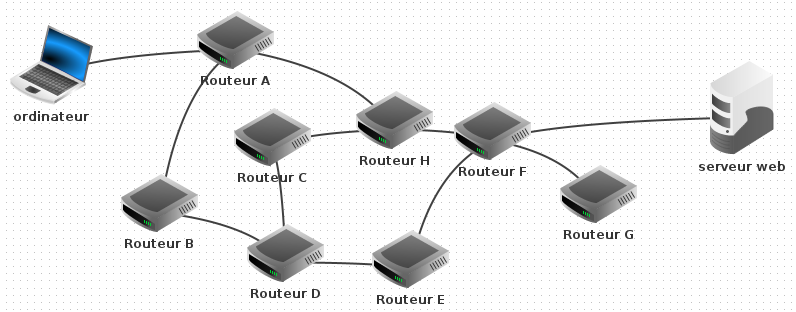
\includegraphics[width=10cm]{ressources/maille.png}
        \captionof{figure}{\centering \textbf{Réseau maillé: }Les routeurs son connectés entre eux pour former une \textbf{toile}}
        \label{IMG}
        \end{center}

\end{frame}
\begin{frame}
    \frametitle{}

    \begin{activite}
    \begin{enumerate}
        \item Simuler la structure maillée.
        \item Déterminer les avantages et les inconvénients de ce type de réseau.
    \end{enumerate}
    \end{activite}

\end{frame}
\begin{frame}
    \frametitle{}

    \begin{aretenir}[]
    Un réseau maillé est plus difficile à mettre en place. De plus il est plus coûteux. Cependant la redondance des connexions permet de garantir la transmission des informations.
    \end{aretenir}

\end{frame}
\subsection{Connexion entre réseaux}
\begin{frame}
    \frametitle{Connexion entre réseaux}

    \begin{center}
    \centering
    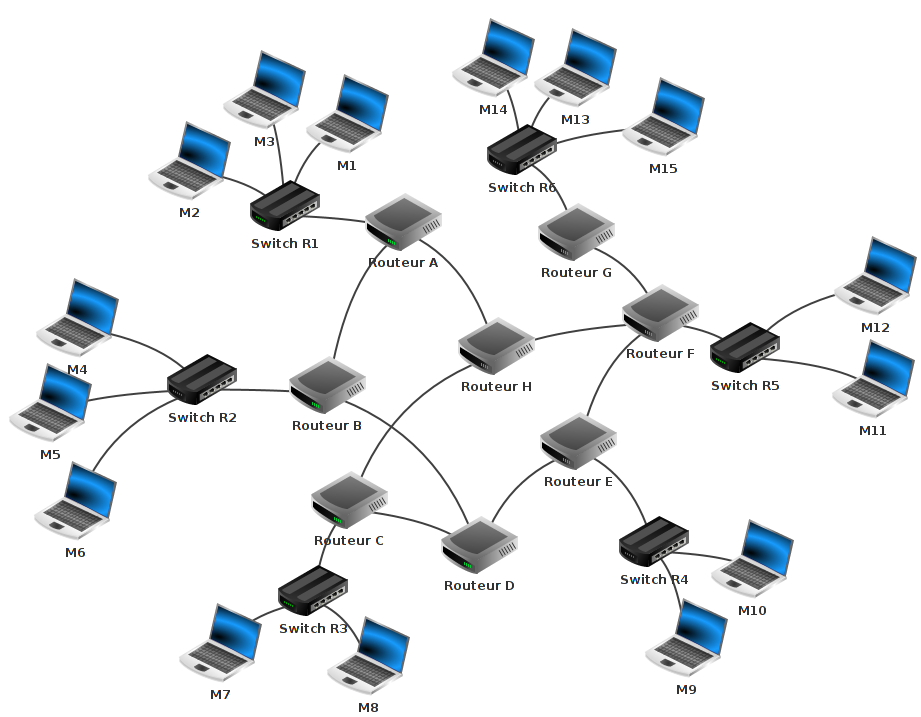
\includegraphics[width=9cm]{ressources/routage.png}
    \captionof{figure}{\centering Le réseau Internet est surnommé le réseau des réseaux.}
    \label{IMG}
    \end{center}

\end{frame}
\begin{frame}
    \frametitle{}

    \begin{aretenir}[]
    Le réseau Internet est une structure maillée qui relie des réseaux plus petits. Un \emph{petit} réseau peut contenir plusieurs centaines de machines.
    \end{aretenir}

\end{frame}
\end{document}